%% ----------------------------------------------------------------
%% Thesis.tex -- MAIN FILE (the one that you compile with LaTeX)
%% ---------------------------------------------------------------- 

% Set up the document
\documentclass[11pt]{article}

\usepackage{setspace}
\setlength{\parskip}{1ex}
\setlength{\topmargin}{-0.5in}
\setlength{\oddsidemargin}{+.1in}
\setlength{\evensidemargin}{-.2in}
\setlength{\textheight}{9in}
\setlength{\textwidth}{6.5in}
\usepackage[paper=a4paper,margin=1in]{geometry}

% Include any extra LaTeX packages required
\usepackage[square, numbers, comma, sort&compress]{natbib}  % Use the "Natbib" style for the references in the Bibliography
\usepackage{verbatim}  % Needed for the "comment" environment to make LaTeX comments
\usepackage{vector}  % Allows "\bvec{}" and "\buvec{}" for "blackboard" style bold vectors in maths

\usepackage{sectsty}

\usepackage{titlesec}

\titleformat{\chapter}[display]   
{\normalfont\normalsize\bfseries}{\chaptertitlename\ \thechapter}{1pt}{\normalsize}   
\titlespacing*{\section}{0pt}{-8pt}{-10pt}

\chapternumberfont{\normalsize}
\chaptertitlefont{\normalsize}
\sectionfont{\small}



%% ----------------------------------------------------------------
\begin{document}
%\frontmatter      % Begin Roman style (i, ii, iii, iv...) page numbering

% Set up the Title Page
\title  {Kotlin Research}
%\authors  {\texorpdfstring
%            {\href{btsibu@oakland.edu}{Blair Sibu}}
            {Blair Sibu}
%            }
%\addresses  {\deptname\\\univname}  % Do not change this here, instead these must be set in the "Thesis.cls" file, please look through it instead
\date       {\today}
%\subject    {}
%\keywords   {}

\maketitle
%% ----------------------------------------------------------------

% Define the page headers using the FancyHdr package and set up for one-sided printing
%\fancyhead{}  % Clears all page headers and footers
%\rhead{\thepage}  % Sets the right side header to show the page number
%\lhead{}  % Clears the left side page header

%\pagestyle{fancy}  % Finally, use the "fancy" page style to implement the FancyHdr headers

%% ----------------------------------------------------------------

%\pagestyle{fancy}  %The page style headers have been "empty" all this time, now use the "fancy" headers as defined before to bring them back

%% ----------------------------------------------------------------
%\mainmatter	  % Begin normal, numeric (1,2,3...) page numbering
  % Return the page headers back to the "fancy" style

% Include the chapters of the thesis, as separate files
% Just uncomment the lines as you write the chapters


\begin{center}
\section{Efficiency}
\end{center}
\hspace{1em}Kotlin is a statically typed programming language. This means that the type of variable is known at compile time. However, even though it uses Java libraries to compile it is different in how it specifies its variable type. In Java each variable type must be specified, but in Kotlin it has a way to deduce the type of the variable. 

\subsection{JIT Compiler}
\hspace{1em}Since Kotlin relies heavily on Java libraries it also uses its Just-In-Time (JIT) compiler. The JIT compiler improves performance at runtime and converts the code into Java byte code contained in a .class file. On start-up thousands of methods need to be called which slows down initial compilation time. Even though it's calling thousands of methods, JIT keeps a strict track of how much memory it is using to avoid an overflow. Once it uses up its maximum cache the JIT compiler stops compiling methods. 

\subsection{Type Casting}
\hspace{1em}Unlike Java, Kotlin can do type casting automatically on compilation. This would be a problem since it could hide some type compatibility errors, but Kotlin only automatically casts something when there is no other possible type to cast a variable to. One thing that cannot be done with Kotlin is assign primitive type to more complex types. In this case, they do not automatically type cast upon compilation. For example, \\$val=x:Int = 20$, $val=y:Long =x$ will not compile. We must use a toLong() dot operator to x to explicitly convert it to a long type instead.

\subsection{Compiler Time}
\hspace{1em}When looking at Java v. Kotlin for Android Development it is only slower on clean builds of an app. On average Kotlin compiles slightly faster with incremental compilation.
\vspace{1em}
\begin{center}
	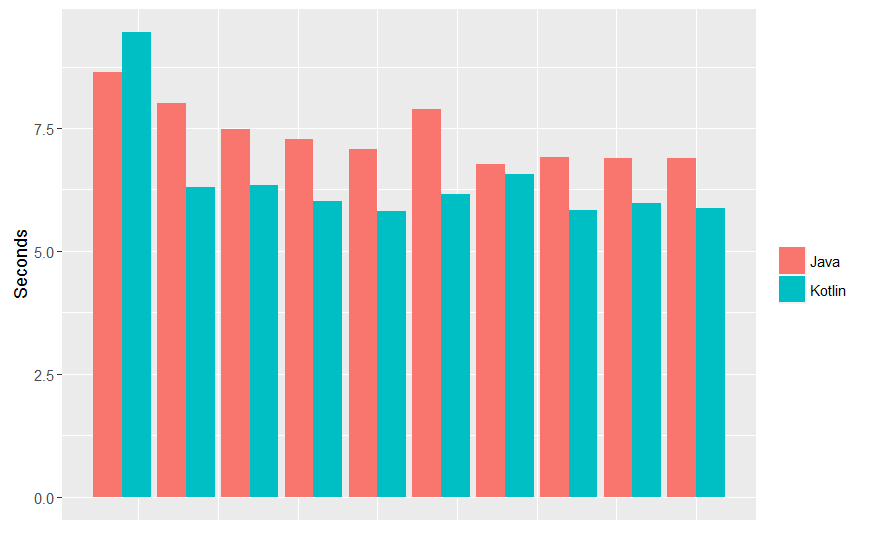
\includegraphics[scale=0.3]{kot}
	\\
	incremental builds with 1 core file changed 
\end{center} % Efficiency

\textbf{\title{\large{Simplicity}}}

\hspace{1em}For the readability and writability of Kotlin it is much easier than Java. The declaring of variables almost looks like javascript, and to declare and object the `new' keyword isn't needed. Kotlin takes all of the code that can be written in Java and condenses it down in an almost shorthand-like form.

\section*{Writability}
\hspace{1em}As stated earlier Kotlin takes a lot less code than Java does. For instance in Java to code a Plain Old Java Object (POJO) with getters, setters, equals(), hascode(), toString(), and copy it takes more than twenty lines of code. With Kotlin we can simply make the POJO in one line: \texttt{data class Person(var name: String, var age: Int)}. With the person class in place a person can be created like so: \texttt{val jack = Person(name = "Jack", age = 20)}. There is no need to use the `new' keyword to create a POJO. Using the Java classes also gives it an advantage of being able to use all the things that Java can use such as maps and arraylists, so it brings the familiarity of Java in being able to write it easily. There are some more extreme sides to Kotlin. In Kotlin you cannot override a class or function unless it's open. Similarly you cannot inherit anything from another class unless it is open. A Good point brought up by Robert C. Martin is that Kotlin is less flexible because its a more statically typed language, even more so than Java, and it puts error checking that would normally be done by the programmer onto the language itself. Although Kotlin manages to compress a lot of unnecessary lines, as stated above, making it a lot easier to write it has some other unfavorable characteristics.

\section*{Readability}
\hspace{1em}Reading Kotlin code is a little bit trickier than writing it. From the code above, \texttt{data class Person(var name: String, var age: int)} it is not clear that this is creating a POJO unless that information is known beforehand. Also many languages use the `?' ternary operator, and so does Kotlin, but it also uses it for its Null Safety feature. So depending on the context it could become a little confusing. There are some things that bring a little familiarity to a programmer, for example to declare variables the `var' keyword is used. This is the same exact way local variables are created in C\# and Javascript. In order to make constants easier to read they have allowed underscores to be used, for example if we have a credit card number it could be declared as: \\$val$ $creditCardNumber = 1234\_5678\_9012\_3456L$ where L indicates that it is of type long and val is the equivalent of `final' in Java. The creators of Kotlin have also taken a page out of python's book by using the keyword `in.' This makes the foreach loop more readable: \texttt{for(c in arr)}. Despite the few things that Kotlin does that make it confusing at times it reads a lot like other languages would. It takes on a lot of characteristics that Javascript, Java, and Python have. In doing so it is easier to read than Java.

 % Simplicity

\begin{center}
\section{Orthogonality}
\end{center}

\hspace{1em}Kotlin has a relatively small set of primitives; they are the ones that we would expect from Java, integers, booleans, characters, floats, etc. It also uses the same kinds of data structures as Java such as the Array class. The Array class can be used as expected, that is it can be used with all of the primitive types like so: \texttt{Array<TYPE>}. Maps, Lists, etc can be used in the same way. This leaves us with fairly regular amount of Orthogonality. Since Kotlin is so concisely typed there is only one way in which we can declare these structures. [need to write more here] % Orthogonality

\textbf{\title{\normalsize{Definiteness}}}
\section*{Syntax and Semantics}
\hspace{1em} If we compare the syntax of Kotlin to Java almost everything is entirely new. Instead of declaring a variable with its data type, like a lot of the strongly typed languages, Kotlin starts the declaration with either val or var. Val means that the value the variable takes on is immutable while var is mutable. One plain example in how things are declared is the declaration of primitive arrays, that is arrays that are not declared using the Array class: \textit{val x: IntArray = intArrayOf(1, 2, 3)}; which means the value x, which is immutable, is an integer array containing the values 1, 2, and 3. Values from this array can be called as expected, x[0]. Also all of the types (int, boolean, double, etc) are declared after the variable name. However, as stated previously there are times where we do not need to declare the type of the variable because the compiler can infer. 

\hspace{1em} Kotlin also uses the `?' operator to check if something will output a null, or simply to box variables into say the java.lang.Integer class: \textit{val bob?.department} or \textit{val a: Int? = 1} respectively. The first one checks to see if bob is in a department, if he is it will return the value of the department otherwise it will return null. For the second one it is checking to see if the following number can safely be boxed into the java.lang.Integer class. Another useful syntax is when an argument has to call upon a range of numbers, \textit{if(c in 0..9)}. When there's an argument that is searching through a range of numbers it simply means that if the c is in the range from zero to nine, then execute. The range can be used in any conditional statement. `!in' could also be used which is the negation of the `in.'

\hspace{1em}For many other structures, if-else, while, for, etc they are all written the same as in Java. Looking back at the example of the foreach loop \textit{for(c in str)}, this means precisely that for each element c, that is for each character, in the string variable str. So the loop will loop as long as a character remains in the string str. Since there are many primitive types there are also many ways to convert them, for example if an argument needed a long but instead the variable was an integer it could be changed with the following: \textit{x.toLong()} assuming that x is an integer. This can also be done with strings to characters or a numerical to a character. A function can be define with the keyword `fun.' It is much like a method in Java and it takes input quite the same way, for example \textit{fun printer(str: String)}. This function is named printer and take a string input. For anything that is syntactically the same in Kotlin as it is in Java, the semantics are also the same. % Definiteness


\begin{center}
\section{Reliability}
\end{center}

\hspace{1em} Kotlin has just as much reliability as Java does and more. With Kotlin there's the Null safety feature which protects us against the null pointer value exception. It also uses the try catch blocks as well as the throwable Java class. 

\subsection{Null Safety}

\hspace{1em}Kotlin tries to get rid of Java's NullPointerException error. To do this Kotlin explicitly tells the system which references can hold null. It does this with the `?' ternary operator. For example, \textit{var b: String? = "abc"}, if at any point the variable b becomes null it's ok because it has been allowed to be nullable. However, this does not mean that error checking still doesn't have to be done. If b does happen to become null and later on in the program it's using b.length, then the program must first check if b is null before performing the length command. This can be done like so, \textit{if(b != null) b.length)}. Although instead of checking it to be null there's another operator, `!!'. This operator says that the variable has to strictly be non-null to perform the operation, otherwise it returns a NullPointerException.

\subsection{Exceptions}

\hspace{1em} One thing that Kotlin improves upon in its language is that it does not have checked exceptions. This cuts down on the code that is needed to handle exceptions and also lessens the overhead of checked exceptions. As expected Kotlin also has keywords such as, `throw' so that exception objects can be thrown. It also has the try catch blocks for catching and handling exceptions.

 % Reliability

\textbf{\title{\normalsize{Program Verification}}}
\section{Correctness}
[talk about assertions and what not. I believe you can also use maven/JUnit] % Correctness

\textbf{\title{\normalsize{Abstraction Facilities}}}

\section{Data}

\section{Procedural} % Abstraction Facilities

%% ----------------------------------------------------------------
% Now begin the Appendices, including them as separate files


%\input{Appendices/AppendixB} % Appendix Title

%\input{Appendices/AppendixC} % Appendix Title

%% ----------------------------------------------------------------

\end{document}  % The End
%% ----------------------------------------------------------------